\begin{knitrout}
\definecolor{shadecolor}{rgb}{0.969, 0.969, 0.969}\color{fgcolor}\begin{figure}
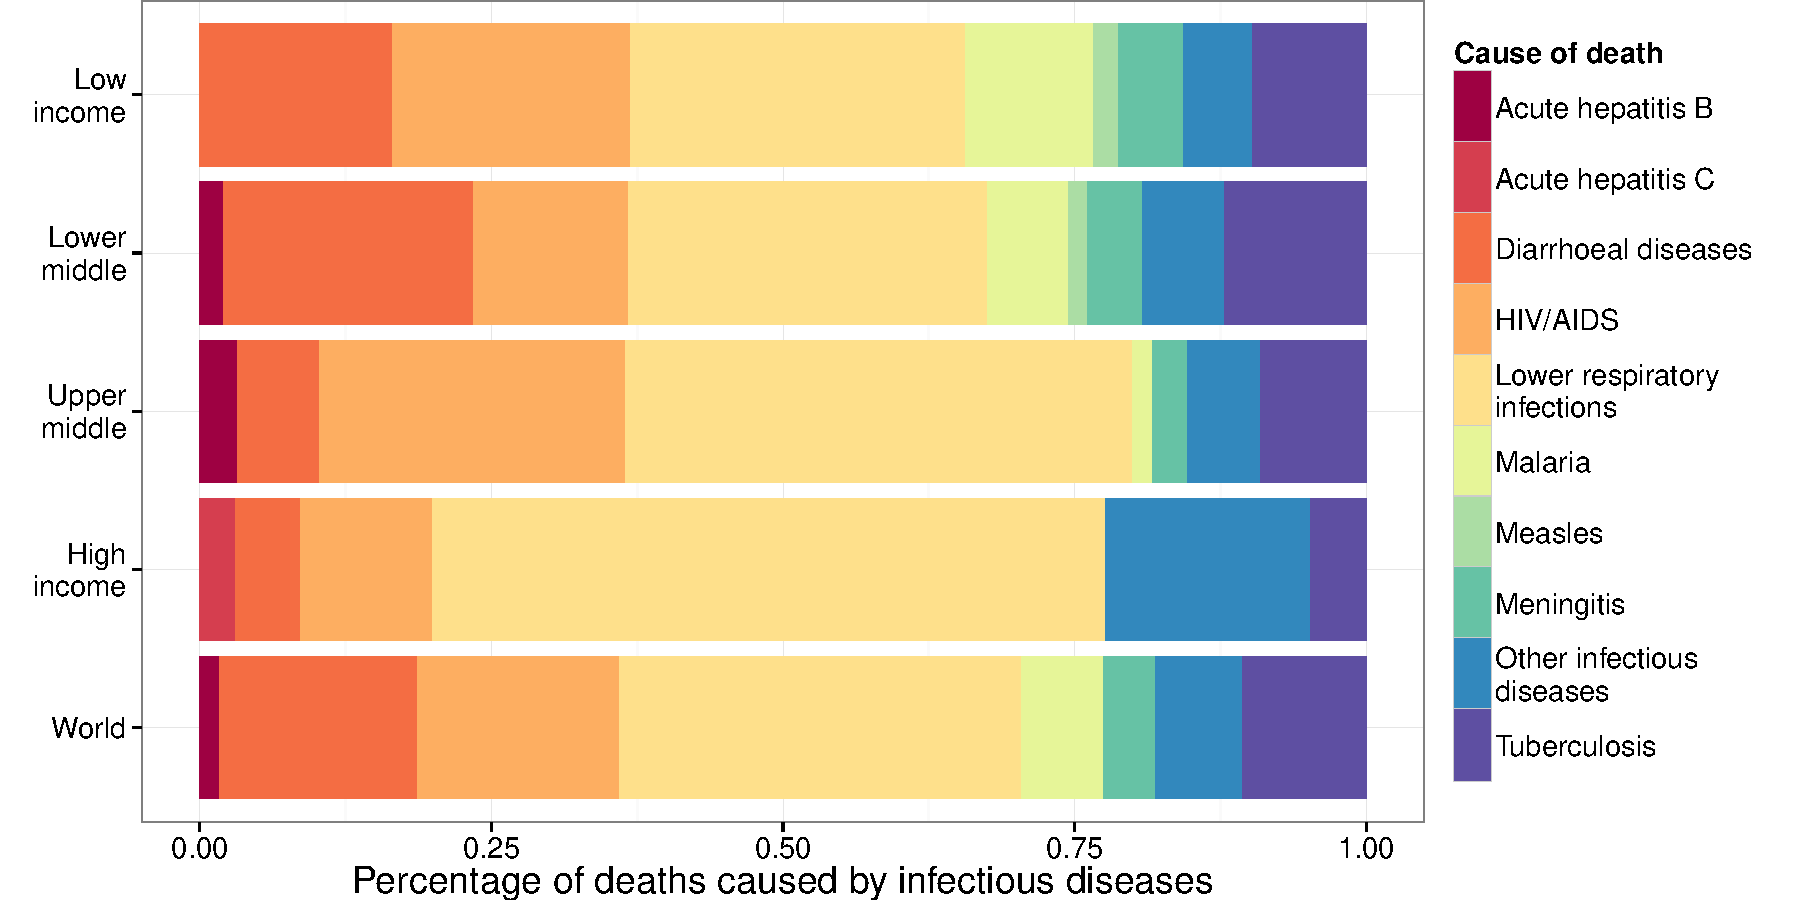
\includegraphics[width=\maxwidth]{figures/R/who-deaths/byDisease-who-deaths_by-disease-1} \caption{Relative frequencies of death causes in 2012 by World Bank income groups. Binning is based on Gross National Income (GNI; see figure \ref{fig:who-deaths_top-causes}). The data was obtained from the \cite{WHO2012}.}\label{fig:who-deaths_by-disease}
\end{figure}


\end{knitrout}

\newcommand{\knitrPercentageInfectTwelveWorldLRI}{34.5\%}
\newcommand{\knitrPercentageInfectTwelveHighLRI}{57.7\%}
\newcommand{\knitrPercentageInfectTwelveUmidLRI}{43.5\%}
\newcommand{\knitrPercentageInfectTwelveLmidLRI}{30.8\%}
\newcommand{\knitrPercentageInfectTwelveLowLRI}{28.7\%}
\newcommand{\knitrPercentageInfectTwelveHighDiarr}{5.6\%}
\newcommand{\knitrPercentageInfectTwelveUmidDiarr}{7\%}
\newcommand{\knitrPercentageInfectTwelveLmidDiarr}{21.4\%}
\newcommand{\knitrPercentageInfectTwelveLowDiarr}{16.6\%}
\newcommand{\knitrPercentageInfectTwelveWorldAIDS}{17.3\%}
\newcommand{\knitrPercentageInfectTwelveWorldDiarr}{16.9\%}
\newcommand{\knitrPercentageInfectTwelveHighAIDS}{11.3\%}
\newcommand{\knitrPercentageInfectTwelveUmidAIDS}{26.2\%}
\newcommand{\knitrPercentageInfectTwelveLmidAIDS}{13.3\%}
\newcommand{\knitrPercentageInfectTwelveLowAIDS}{20.4\%}
